\documentclass[crop,tikz]{standalone}
\usetikzlibrary{backgrounds}
\colorlet{blue}{cyan}
\tikzset{
  inverted/.style = {
    every path/.style = {draw=white,text=white},
    background rectangle/.style={fill},
    show background rectangle
  }
}

\tikzset{>=latex}
\usetikzlibrary{calc,decorations.markings,shapes}
\colorlet{gray}{gray!60}
\colorlet{green}{green}

\begin{document}
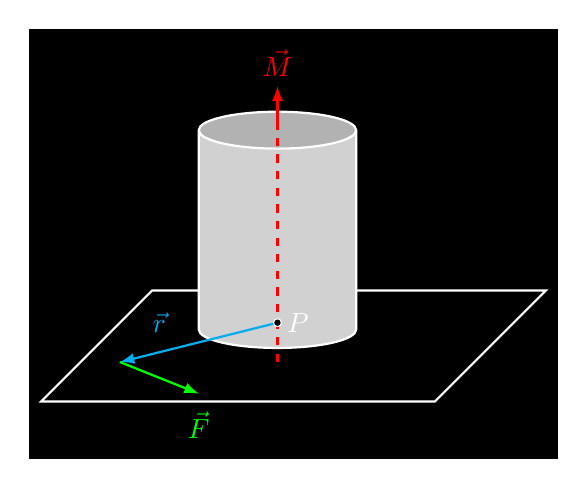
\begin{tikzpicture}[inverted,inverted]
  \draw[thick] (-3cm,-2cm) -- ++(5cm,0) -- ++(1.41cm,1.41cm) -- ++(-5cm,0) -- cycle;
  \node (A) at (0,0) [thick, cylinder, aspect=2, shape border rotate=90, draw, minimum height=3cm, minimum width=2cm, cylinder body fill=gray!60, cylinder uses custom fill, cylinder end fill=gray] {};
  \draw[dashed,red,thick] (0,-1.5cm) -- (0,1.5cm);
  \draw[->,red,thick] (0,1.5cm) -- +(0,0.5cm) node[above] {$\vec{M}$};
  \coordinate (C) at (0,-1cm);
  \coordinate (R) at ($(C)+(-2cm,-0.5cm)$);
  \draw[->,blue,thick] (C) -- node[above,xshift=-0.5cm] {$\vec{r}$} (R);
  \draw[->,green,thick] (R) -- +(1cm,-0.4cm) node[below,yshift=-0.1cm] {$\vec{F}$};
  \draw[fill] (C) circle (0.05cm) node[right] {$P$};
\end{tikzpicture}
\end{document}
